\documentclass{beamer}

\setbeamertemplate{navigation symbols}{}
\setbeamertemplate{footline}[15]
\setbeamercolor{title}{fg=white,bg=darkred!80!black}
\usetheme{CambridgeUS}
\setcounter{MaxMatrixCols}{12}

\title[Repressilator]{Repressilator: simulation and analysis of a synthetic oscillatory network in \textit{E. coli}}
\author{Daniel S. Standage}
\date{\today}
\institute[BCB 570]{BCB 570}

\begin{document}
 

\begin{frame}
  \titlepage
\end{frame}

\section{Background}
\subsection{Repressilator}
\begin{frame}
  \frametitle{Repressilator}
  \begin{center}
    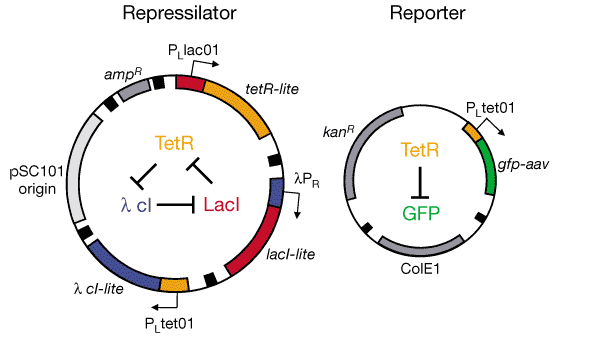
\includegraphics[width=300px]{../repressilator.png}
  \end{center}
\end{frame}
\begin{frame}
  \frametitle{Repressilator}
  \begin{center}
    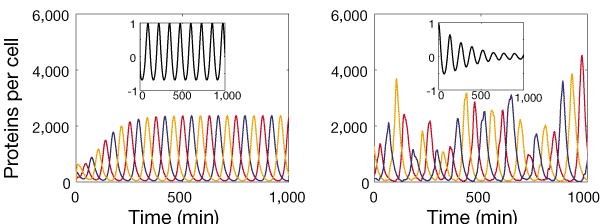
\includegraphics[width=300px]{../simulation.png}
  \end{center}
\end{frame}

\section{Simulation}
\subsection{Gillespie's Algorithm}
\begin{frame}
  \frametitle{Stoichiometric matrix}
  \[ V = 
  \begin{bmatrix}
  1 & 0 & -1 & 0 & 0 & 0 & 0 & 0 & 0 & 0 & 0 & 0 \\
  0 & 1 & 0 & -1 & 0 & 0 & 0 & 0 & 0 & 0 & 0 & 0 \\
  0 & 0 & 0 & 0 & 1 & 0 & -1 & 0 & 0 & 0 & 0 & 0 \\
  0 & 0 & 0 & 0 & 0 & 1 & 0 & -1 & 0 & 0 & 0 & 0 \\
  0 & 0 & 0 & 0 & 0 & 0 & 0 & 0 & 1 & 0 & -1 & 0 \\
  0 & 0 & 0 & 0 & 0 & 0 & 0 & 0 & 0 & 1 & 0 & -1 
  \end{bmatrix}
  \]
\end{frame}
\begin{frame}
  \frametitle{Reactions}
  \begin{itemize}
    \item transcription: \[a_{tr}^0 + \frac{a_{tr} (K_m)^n}{(K_m)^n+I^n}\]
    \item translation: \[k_{tl} T\]
    \item mRNA degredation: \[kd_t T\]
    \item protein degredation: \[kd_p P\]
  \end{itemize}
\end{frame}
\begin{frame}
  \frametitle{Simulation}
  \begin{center}
    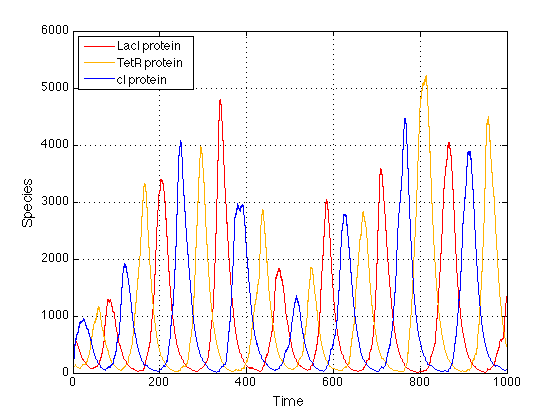
\includegraphics[width=250px]{../results.png}
  \end{center}
\end{frame}

\section{Network analysis}
\subsection{Network analysis}
\begin{frame}
  \frametitle{Network analysis}

\begin{eqnarray*}
D_{tetR} + 2 P_{lacI} &\rightarrow& F_{tetR} \\
             F_{tetR} &\rightarrow& H_{tetR} + P_{lacI} \\
             H_{tetR} &\rightarrow& D_{tetR} + P_{lacI} \\
                      &\rightarrow& R_{tetR} \\
                      &\rightarrow& R_{tetR} \\
                      &\rightarrow& P_{tetR} \\
             R_{tetR} &\rightarrow& \\
             P_{tetR} &\rightarrow& \\
\end{eqnarray*}

\end{frame}
\begin{frame}
  \frametitle{Network analysis}
  \begin{itemize}
    \item<1-> elementary flux modes: 6, 12
    \item<2-> each is an extreme pathway
    \item<3-> flux optimization uninformative
    \item<4-> minimal cut sets: 64, 1728
    \item<5-> simple network, not very informative
  \end{itemize}
\end{frame}

\section{Acknowlegements}
\begin{frame}
  \frametitle{Thanks to...}
  \begin{itemize}
    \item Will
    \item Tasos
  \end{itemize}  
\end{frame}

\end{document}
